\documentclass[12pt]{article}
\usepackage{blindtext}
\usepackage[en,bordered]{uni-style}
\usepackage{uni-math}
\usepackage{physics}
\usepackage{amssymb}
\usepackage{capt-of}
\title{Intruduction to Machine Learning}
\prof{Dr \,S.Amini}
\subject{Project}
\info{
    \begin{tabular}{lr}
        Amirreza Velae & 400102222\\
        github    & \href{https://github.com/amirrezavelae}{repository}\\
    \end{tabular}
    }
    \date{\today}
    % \usepackage{xepersian}
    % \settextfont{Yas}
    \usepackage{uni-code}
    
\begin{document}
\maketitlepage
\maketitlestart

\section{Theory Questions}
\subsection{Theory Question 1.}
In your own words, explain how the MM algorithm can deal with non-convex optimization objective functions by considering simpler convex objective functions.
\begin{qsolve}[solution]
    MM algorithm is an iterative algorithm for optimizing a nonconvex or nonconcave $l(\theta)$ that has a complex form. For example if our goal is finding maximum of a function we can consider a simpler concave function $Q(\theta,\theta^{(t)})$ that depends on a certain parameter. Function must be tight lowerbound that means in a certain point $l(\theta^{(t)}=Q(\theta^{(t)},\theta^{(t)}))$ and also $l(\theta\leq Q(\theta,\theta^{(t)}))$. In each iteration we choose the max of $Q(\theta,\theta^{(t)}))$ as next level parameter $\theta^{(t+1)}=argmax_{\theta}Q(\theta,\theta^{(t)})$ and we move on to reach the maximum of the main function $l(\theta)$ and according to the following inequality
    we act correctly:
    \\$l(\theta^{(t+1)})\leq Q(\theta^{(t+1)},\theta^{(t)})\leq Q(\theta^{(t)},\theta^{(t)})=l(\theta^{(t)})$
    also we can do same for finding minimum but with convex function.
\end{qsolve}

\subsection{Theory Question 2.}
Briefly explain how the formula for mixture models:
\begin{equation}
    p(y_n;\theta)=\sum_{k=1}^{K}p_Z(z_k;\theta)p_{Y|Z}(y|Z=z_k;\theta)
\end{equation}
is the same as the sum over all possible values of $Z^{(i)}$ in equation
\begin{equation}
    ln(p_Y(y_n;\theta))=\sum_{i=1}^N ln(p(y^{(i)}_n;\theta))=\sum_{i=1}^N ln(\sum_{k=1}^{K}p_{Y,Z}(y^{(i)}_n,z^{(i)}_n=k;\theta))
\end{equation}
Explain why it’s easier to optimize $p_{Y,Z}(y^{i}_n,z^{i}_n=K;\theta)$ than $p(y_n;\theta)$ in the context of mixture models.
\begin{qsolve}[solution]
    The model is simplified by Bayes' rule:
    \\$p(y,z)=p(y|z)p(z)$
        \\$p(y_n;\theta)=\sum_{z_n}p_{Y,Z}(y_n,z_n;\theta)=\sum_{k=1}^{K}p_Z(z_k;\theta)p_{Y|Z}(y|Z=z_k;\theta)$
    \\It is easier to optimize $p_{Y,Z}(yn, zn; θ)$ because in this case we know which distribution each data belongs to so optimizing become easier because we can optimize each distribution separately and find the parameters of each one.
    \\But it is hard to optimize if we just know that a data comes from sumation of some distribution and don't know anything about each distribution because we can not fit a single distribution to model.
\end{qsolve}



\subsection{Theory Question 3.}
Read about variational inference (or variational bayesian methods) and compare it with the procedure we used for the EM algorithm (You might want to check Wikipedia for this!)
\begin{qsolve}[solution]
    Variational Bayes (VB) is often compared with expectation maximization (EM). The actual numerical procedure is quite similar, in that both are alternating iterative procedures that successively converge on optimum parameter values. The initial steps to derive the respective procedures are also vaguely similar, both starting out with formulas for probability densities and both involving significant amounts of mathematical manipulations. However, there are a number of differences. Most important is what is being computed. EM computes point estimates of posterior distribution of those random variables that can be categorized as "parameters", but only estimates of the actual posterior distributions of the latent variables (at least in "soft EM", and often only when the latent variables are discrete). The point estimates computed are the modes of these parameters; no other information is available. VB, on the other hand, computes estimates of the actual posterior distribution of all variables, both parameters and latent variables. When point estimates need to be derived, generally the mean is used rather than the mode, as is normal in Bayesian inference. Concomitant with this, the parameters computed in VB do not have the same significance as those in EM. EM computes optimum values of the parameters of the Bayes network itself. VB computes optimum values of the parameters of the distributions used to approximate the parameters and latent variables of the Bayes network. For example, a typical Gaussian mixture model will have parameters for the mean and variance of each of the mixture components. EM would directly estimate optimum values for these parameters. VB, however, would first fit a distribution to these parameters — typically in the form of a prior distribution, e.g. a normal-scaled inverse gamma distribution — and would then compute values for the parameters of this prior distribution, i.e. essentially hyperparameters. In this case, VB would compute optimum estimates of the four parameters of the normal-scaled inverse gamma distribution that describes the joint distribution of the mean and variance of the component.
\end{qsolve}
\clearpage

\section{Simulation Questions}
Libraries used in phase1 are:
\begin{itemize}
    \item $numpy$
    \item $pandas$
    \item $matplotlib$
    \item from $scipy.stats$ import $multivariate\_normal$
\end{itemize}
code is in \href{https://github.com/amirrezavelae/Introduction-to-Machine-Learning/blob/master/IML_Project/Phase1/code.ipynb}
\subsection{Simulation Question 1.}
Each distribution has 200 data points that are concatenated in a two-dimensional array and given to you. Plot the data with three different colors in a graph.
\begin{qsolve}
    \begin{lstlisting}[language=Python,caption={Simulation Question 1.},label={code:Simulation Question 1.}]
#plot data function
def plot_data(name):
    #read data
    data = pd.read_csv(name+'.csv',header=None)

    #split data into 3 arrays
    data1 = data.iloc[0:200,1:3]
    data2 = data.iloc[200:400,1:3]
    data3 = data.iloc[400:600,1:3]

    #convert to numpy array
    data1 = data1.to_numpy()
    data2 = data2.to_numpy()
    data3 = data3.to_numpy()

    #plot the data
    plt.scatter(data1[:,0],data1[:,1],color='red', label='class1')
    plt.scatter(data2[:,0],data2[:,1],color='blue', label='class2')
    plt.scatter(data3[:,0],data3[:,1],color='green', label='class3')
    plt.xlabel('x1')
    plt.ylabel('x2')
    plt.title(name)
    plt.legend()
    plt.show()
#plot data
plot_data('image1')
plot_data('image2')
        \end{lstlisting}

    \splitqsolve
    results are:
    \tcblower
    \centering
    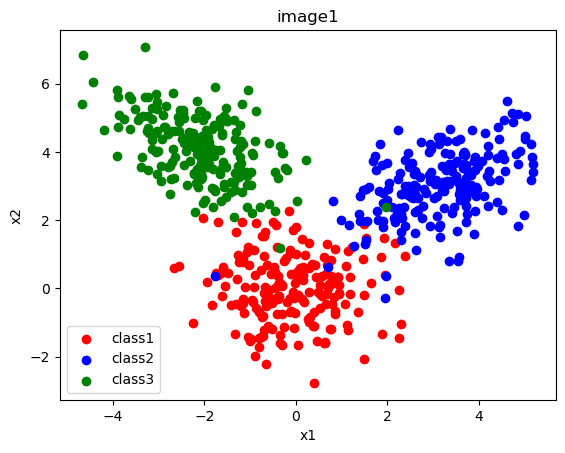
\includegraphics[width=0.4\textwidth]{outputs/output1.png}
    \captionof{figure}{image1 scatter plot}\label{fig:fig1}
    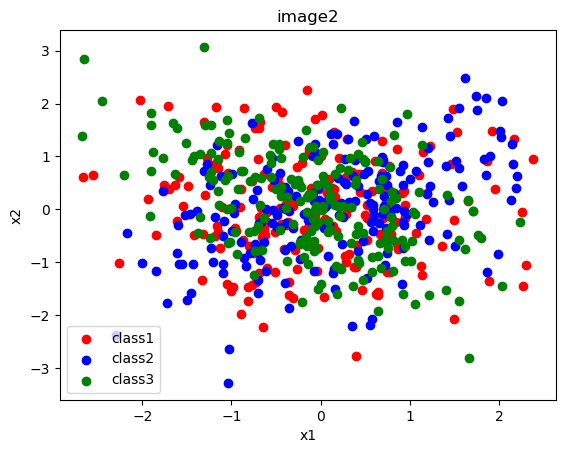
\includegraphics[width=0.4\textwidth]{outputs/output2.png}
    \captionof{figure}{image2 scatter plot}\label{fig:fig2}
\end{qsolve}
\subsection{Simulation Question 2.}
Write a function that performs the E-step. This means assigning each data to a distribution based on the Euclidean distance. Return as output a 3 × 600 array specifying which distribution each data belongs to. If the $R_{ij}$ is one, it means that the $i$–th data is assigned to the $j$–th distribution. Run this function for one iteration and report the result.
\begin{qsolve}
    Function used to perform E-step is:
    \begin{lstlisting}[language=Python,caption={E-step algorithm},label={code:E-step algorithm}]
#E-Step algorithm
def E_step(data, mu, cov, pi,gamma):
    k = mu.shape[0]
    for j in range(k):
        gamma[:,j] = pi[j]*multivariate_normal(mu[j],cov[j]).pdf(data)
    gamma = gamma/gamma.sum(axis=1).reshape(-1,1)
    return gamma
    \end{lstlisting}
    \splitqsolve
    rest of the code is:
    \begin{lstlisting}[language=Python,caption={Simulation Question 2.},label={code:Simulation Question 2.}]
#initialize parameters
def initialize(data, k):
    n = data.shape[0]
    d = data.shape[1]
    pi = np.ones(k)/k
    mu = data[np.random.randint(data.shape[0], size=k), :]
    cov = np.zeros((k,d,d))
    for i in range(k):
        cov[i] = np.eye(d)
    gamma = np.zeros((n,k))
    return pi, mu, cov, gamma

#E-Step algorithm
def E_step(data, mu, cov, pi,gamma):
    k = mu.shape[0]
    for j in range(k):
        gamma[:,j] = pi[j]*multivariate_normal(mu[j],cov[j]).pdf(data)
    gamma = gamma/gamma.sum(axis=1).reshape(-1,1)
    return gamma

#assign each data point to a class
def assign(data, mu, cov):
    k = mu.shape[0]
    n = data.shape[0]
    gamma = np.zeros((n,k))
    for j in range(k):
        gamma[:,j] = multivariate_normal(mu[j],cov[j]).pdf(data)
    gamma = gamma/gamma.sum(axis=1).reshape(-1,1)
    return gamma.argmax(axis=1), gamma

#plot the results
def plot(mu, cov, data,data_class, name):
    #scatter plot of distribution
    x1 = np.linspace(data[:,0].min(),data[:,0].max(),data.shape[0])
    x2 = np.linspace(data[:,1].min(),data[:,1].max(),data.shape[0])
    X, Y = np.meshgrid(x1,x2)
    pos = np.empty(X.shape + (2,))
    pos[:, :, 0] = X; pos[:, :, 1] = Y
    k = mu.shape[0]
    colors = ['red','blue','green']
    for i in range(k):
        Z = multivariate_normal(mu[i],cov[i])
        plt.contour(X, Y, Z.pdf(pos), colors=colors[i], label='class'+str(i+1))
    plt.scatter(data[:,0],data[:,1],color='black', label='data')
    plt.xlabel('x1')
    plt.ylabel('x2')
    plt.title(name)
    plt.legend()
    plt.show()
    plt.scatter(data[:,0],data[:,1],c=data_class, cmap='viridis')
    plt.xlabel('x1')
    plt.ylabel('x2')
    plt.title(name)
    plt.show()
    \end{lstlisting}
    \splitqsolve
    \begin{lstlisting}[language=Python,caption={Simulation Question 2.},label={code:Simulation Question 2.}]
#read data
data1 = pd.read_csv('image1.csv',header=None)
data2 = pd.read_csv('image2.csv',header=None)

#run E-Step algorithm
pi1, mu1, cov1, gamma1 = initialize(data1.iloc[:,1:3].to_numpy(), 3)
pi2, mu2, cov2, gamma2 = initialize(data2.iloc[:,1:3].to_numpy(), 3)

gamma1 = E_step(data1.iloc[:,1:3].to_numpy(), mu1, cov1, pi1,gamma1)
gamma2 = E_step(data2.iloc[:,1:3].to_numpy(), mu2, cov2, pi2,gamma2)



#assign each data point to a class
data1_class , R1 = assign(data1.iloc[:,1:3].to_numpy(), mu1, cov1)
data2_class , R2 = assign(data2.iloc[:,1:3].to_numpy(), mu2, cov2)

plot(mu1, cov1, data1.iloc[:,1:3].to_numpy(),data1_class, 'image1')
plot(mu2, cov2, data2.iloc[:,1:3].to_numpy(),data2_class, 'image2')

def save_R(R, name):
    #set 1 to max of R's row
    R = R == R.max(axis=1)[:,None]
    #save R as 0 and 1 in csv file in output folder
    R = R.astype(int)
    R = pd.DataFrame(R)
    np.savetxt('../Report/outputs/R'+name.replace('image','')+'.csv', R, delimiter=',', fmt='%d')

save_R(R1, 'image1')
save_R(R2, 'image2')
    \end{lstlisting}
    results of plotting data are:
    \tcblower
    \centering
    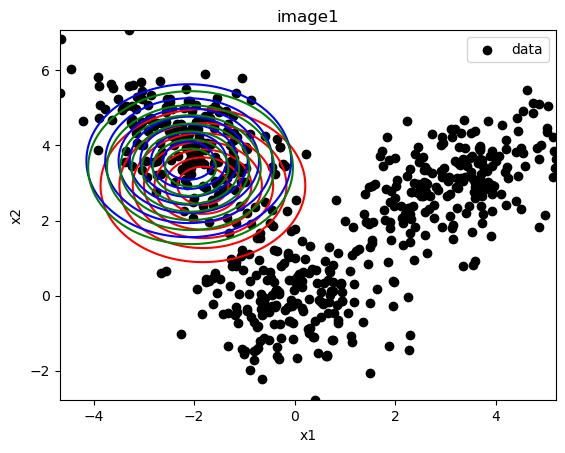
\includegraphics[width=0.4\textwidth]{outputs/output3.png}
    \captionof{figure}{contour plot for estimated distribution after 1 iteration for image1}\label{fig:fig3}
    \splitqsolve
    \centering
    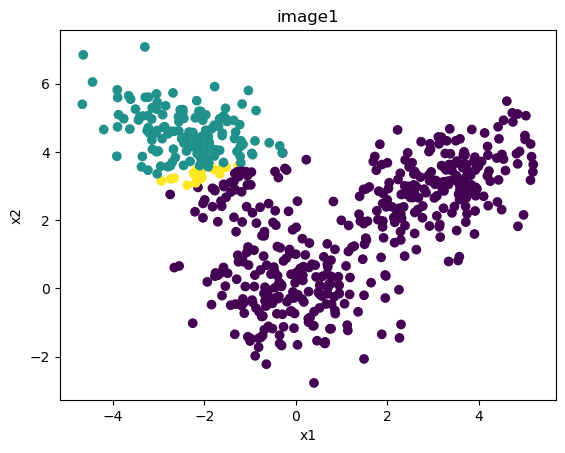
\includegraphics[width=0.4\textwidth]{outputs/output4.png}
    \captionof{figure}{each data point assigned to most possible distribution for image1}\label{fig:fig4}
    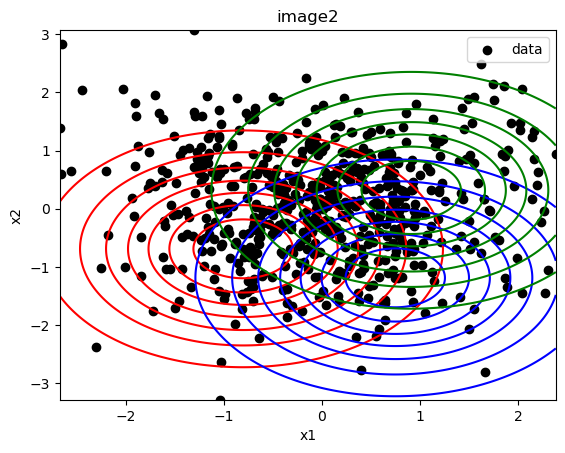
\includegraphics[width=0.4\textwidth]{outputs/output5.png}
    \captionof{figure}{contour plot for estimated distribution after 1 iteration for image2}\label{fig:fig5}
    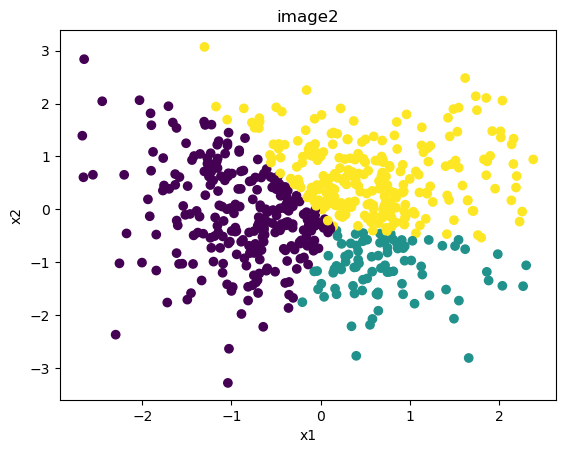
\includegraphics[width=0.4\textwidth]{outputs/output6.png}
    \captionof{figure}{each data point assigned to most possible distribution for image2}\label{fig:fig6}
    \tcblower
    Also R matrix is saved in R1 and R2 as csv file with 0 and 1 in output folder.
\end{qsolve}

\clearpage
\subsection{Simulation Question 3.}
Write a function that performs M-step. This means updating the mean and variance of each distribution. Run this function for one iteration and report the new variances and means of each distribution.
\begin{qsolve}
    Function used to perform M-step is as follows:
    \begin{lstlisting}[language=Python,caption={M-step algorithm},label={code:M-step algorithm}]
#M-step algorithm
def M_step(data, gamma,mu,cov,pi):
    k = gamma.shape[1]
    n = data.shape[0]
    for j in range(k):
        mu[j] = gamma[:,j].dot(data)/gamma[:,j].sum()
        cov[j] = (gamma[:,j]*(data-mu[j]).T).dot(data-mu[j])/gamma[:,j].sum()
        pi[j] = gamma[:,j].sum()/n
    return mu, cov, pi
    \end{lstlisting}
    rest of the code for simulation question 3 is as follows:
    \begin{lstlisting}[language=Python,caption={M-step algorithm},label={code:M-step algorithm}]
#M-step
mu1, cov1, pi1 = M_step(data1.iloc[:,1:3], gamma1,mu1,cov1,pi1)
mu2, cov2, pi2 = M_step(data2.iloc[:,1:3], gamma2,mu2,cov2,pi2)

#print mean and covariance
print('mu1 = ', mu1)
print('-'*50)
print('cov1 = ', cov1)
print('-'*50)
print('mu2 = ', mu2)
print('-'*50)
print('cov2 = ', cov2)
        \end{lstlisting}
    \splitqsolve
    mean and covariance after one iteration for data are:
    \tcblower
    \centering
    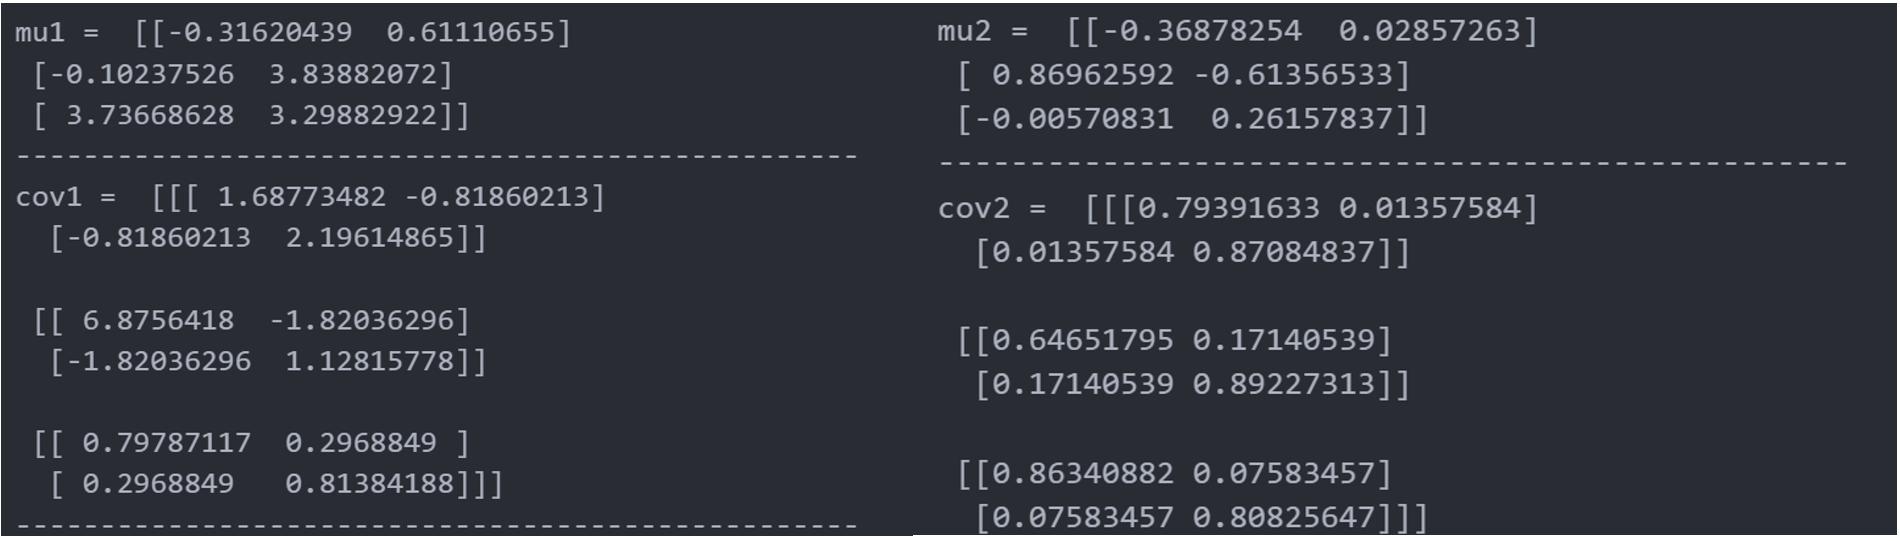
\includegraphics[width=0.8\textwidth]{outputs/output20.png}
    \captionof{figure}{mean and covariance after one iteration for image1 and image2}\label{fig:fig7}

\end{qsolve}

\clearpage
\subsection{Simulation Question 4.}
Using the functions you have written, run the EM algorithm until a convergence is reached or the maximum number of steps is passed. Replot the three new distributions and compare with the correct labels.
\begin{qsolve}
    Function used to apply EM algorithm is as follows:
    \begin{lstlisting}[language=Python,caption={EM algorithm},label={code:EM algorithm}]
        def EM(name,data, k, max_iter):
#initialization
n = data.shape[0]
d = data.shape[1]
pi, mu, cov, gamma = initialize(data, k)
for i in range(k):
    cov[i] = np.eye(d)
gamma = np.zeros((n,k))
log_likelihood = np.zeros(max_iter)
#stop for loop when log_likelihood is not changing or max_iter is reached
for i in range(max_iter):
    #E-step
    gamma = E_step(data, mu, cov, pi,gamma)
    #M-step
    mu, cov, pi = M_step(data, gamma,mu,cov,pi)
    #compute log_likelihood
    log_likelihood[i] = 0
    for j in range(k):
        log_likelihood[i] += np.log(pi[j])*gamma[:,j].sum()
        log_likelihood[i] += gamma[:,j].dot(np.log(multivariate_normal(mu[j],cov[j]).pdf(data)))
    #stop for loop when log_likelihood is not changing or max_iter is reached
    if i > 0:
        if np.abs(log_likelihood[i]-log_likelihood[i-1]) < 1e-7:
            print('log_likelihood for',name,'stopped changing at iteration',i)
            break
return mu, cov, pi, log_likelihood
        \end{lstlisting}
    \splitqsolve
    reest of the code for simulation question 4 is as follows:
    \begin{lstlisting}[language=Python,caption={EM algorithm},label={code:EM algorithm}]
#run EM algorithm
mu1, cov1, pi1, log_likelihood1 = EM('image1',data1.iloc[:,1:3].to_numpy(), 3, 200)
mu2, cov2, pi2, log_likelihood2 = EM('image2',data2.iloc[:,1:3].to_numpy(), 3, 200)

#assign each data point to a class
data1_class , R = assign(data1.iloc[:,1:3].to_numpy(), mu1, cov1)
data2_class , R = assign(data2.iloc[:,1:3].to_numpy(), mu2, cov2)

plot(mu1, cov1, data1.iloc[:,1:3].to_numpy(),data1_class, 'image1')
plot(mu2, cov2, data2.iloc[:,1:3].to_numpy(),data2_class, 'image2')
            \end{lstlisting}
    \splitqsolve

    we plot distributions as contour plots:
    \tcblower
    \centering
    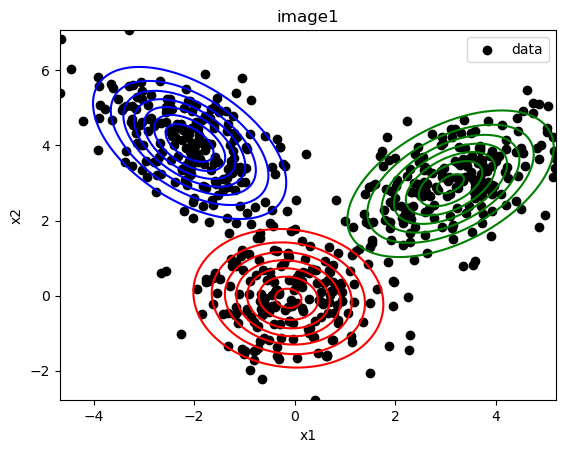
\includegraphics[width=0.4\textwidth]{outputs/output9.png}
    \captionof{figure}{image1 after EM algorithm}\label{fig:fig9}
    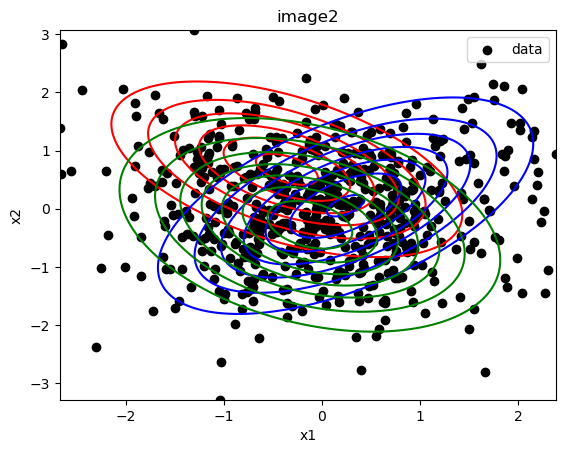
\includegraphics[width=0.4\textwidth]{outputs/output10.png}
    \captionof{figure}{image2 after EM algorithm}\label{fig:fig10}
    \splitqsolve
    also results for plotting classification of image1 and image2 after EM algorithm are as follows:
    \tcblower
    \centering
    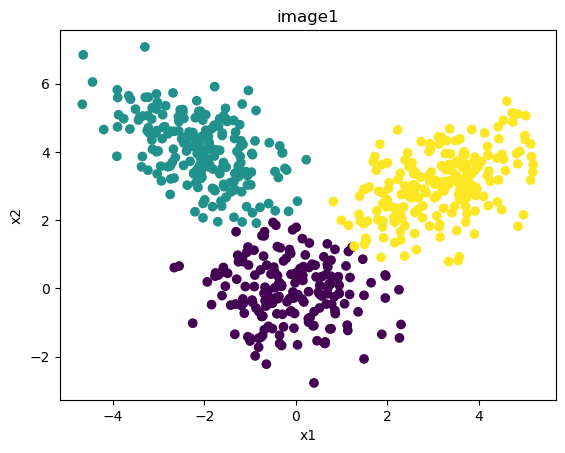
\includegraphics[width=0.4\textwidth]{outputs/output11.png}
    \captionof{figure}{image1 after EM algorithm}\label{fig:fig11}
    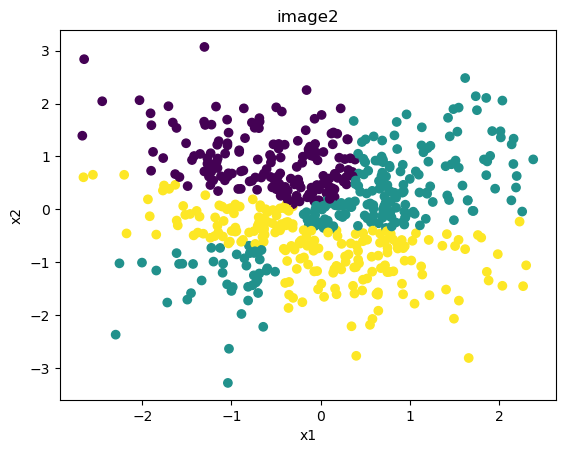
\includegraphics[width=0.4\textwidth]{outputs/output12.png}
    \captionof{figure}{image2 after EM algorithm}\label{fig:fig12}


    \splitqsolve
    to plot NLL and compare with correct labels, we use following code:
    \begin{lstlisting}[language=Python,caption={plot NLL},label={code:plot NLL}]
#plot log_likelihood
plt.plot(log_likelihood1, label='image1')
plt.plot(log_likelihood2, label='image2')
plt.xlabel('iteration')
plt.ylabel('log_likelihood')
plt.title('log_likelihood')
plt.legend()
plt.show()

#plot log_likelihood after 50th iteration
plt.plot(log_likelihood1[50:], label='image1')
plt.plot(log_likelihood2[50:], label='image2')
plt.xlabel('iteration')
plt.ylabel('log_likelihood')
plt.title('log_likelihood after 50th iteration')
plt.legend()
plt.show()
        \end{lstlisting}
    \splitqsolve
    results for plotting NLL are as follows:
    \tcblower
    \centering
    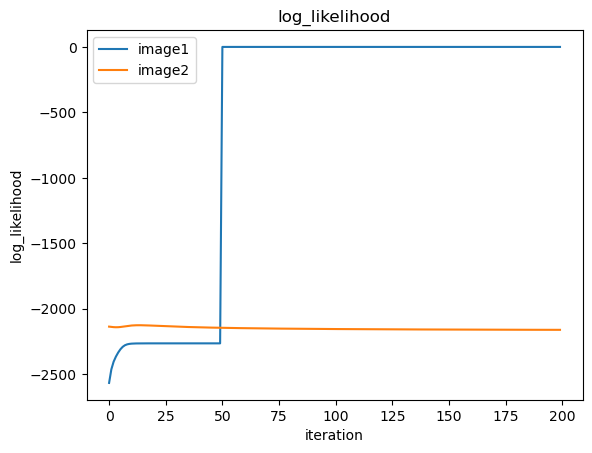
\includegraphics[width=0.37\textwidth]{outputs/output13.png}
    \captionof{figure}{log likelihood}\label{fig:fig13}
    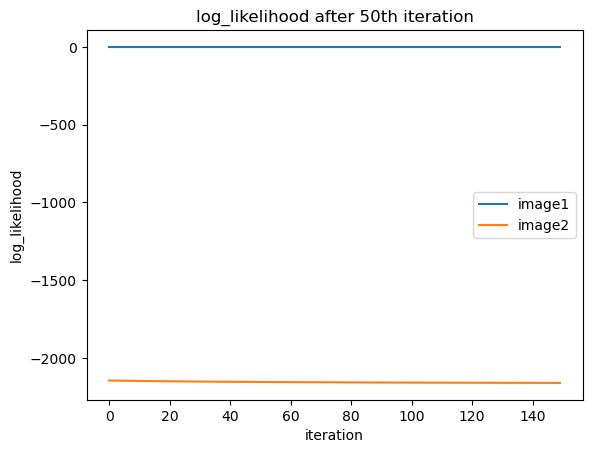
\includegraphics[width=0.37\textwidth]{outputs/output14.png}
    \captionof{figure}{log likelihood after 50th iteration}\label{fig:fig14}
    \splitqsolve

    also, to obtain the new mean and covariance, we use following code:
    \begin{lstlisting}[language=Python,caption={obtain new mean and covariance},label={code:obtain new mean and covariance}]
#print mean and covariance
print('mu1 = ', mu1)
print('-'*50)
print('cov1 = ', cov1)
print('-'*50)
print('mu2 = ', mu2)
print('-'*50)
print('cov2 = ', cov2)
    \end{lstlisting}
    \splitqsolve
    results for new mean and covariance are as follows:
    \tcblower
    \centering
    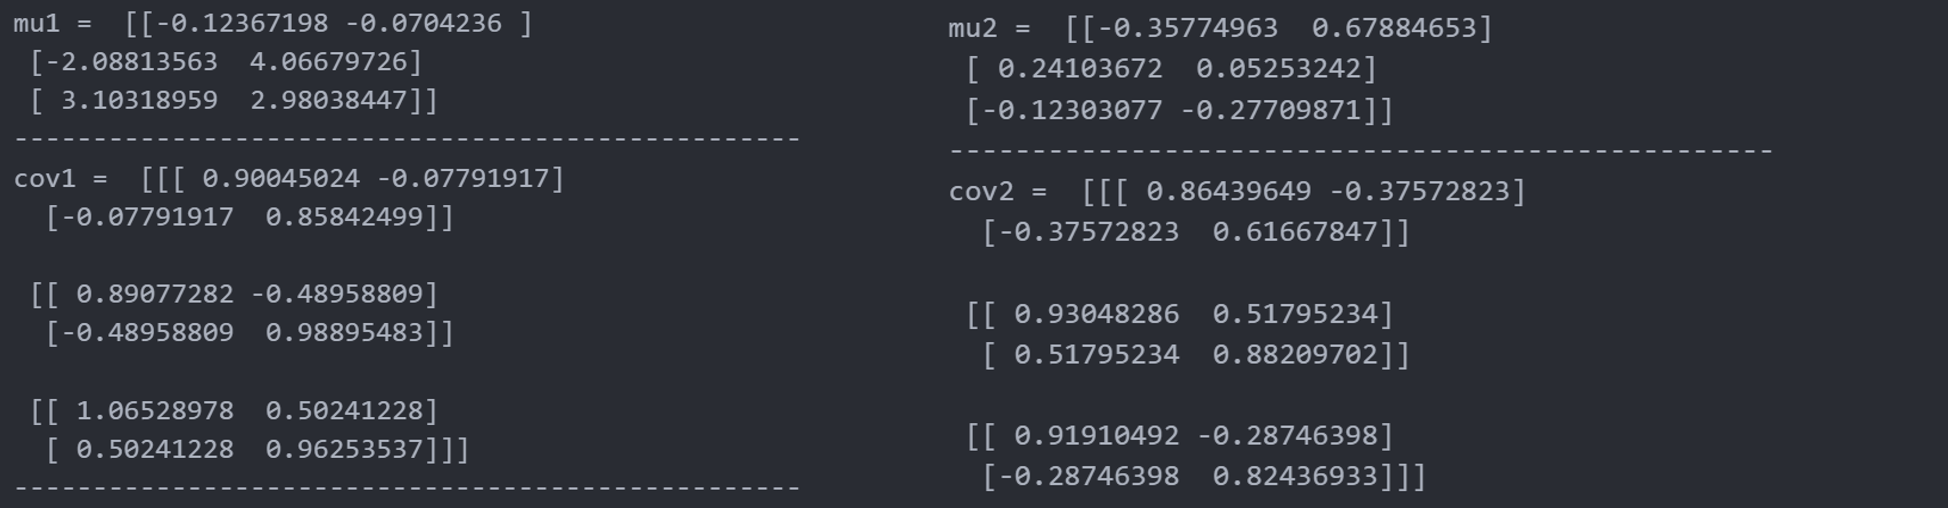
\includegraphics[width=0.7\textwidth]{outputs/output17.png}
    \captionof{figure}{new mean and covariance}\label{fig:fig17}
    \splitqsolve
    to plot misclassified data, we use following code:
    \begin{lstlisting}[language=Python,caption={plot misclassified data},label={code:plot misclassified data}]
#obtain R
data1_class , R1 = assign(data1.iloc[1:601,1:3].to_numpy(), mu1, cov1)
data2_class , R2 = assign(data2.iloc[1:601,1:3].to_numpy(), mu2, cov2)

#plot missclassified data points
def missclassified(data, R,name):
    #set 1 to max of R's row
    R = R == R.max(axis=1)[:,None]
    #save R as 0 and 1
    R = R.astype(int)
    R = pd.DataFrame(R) 
    #find which column has most 1
    a = R.iloc[0:200].sum(axis=0).idxmax()
    b = R.iloc[200:400].sum(axis=0).idxmax()
    c = R.iloc[400:600].sum(axis=0).idxmax()
    #check which column has 1
    for i in range(R.shape[0]):
        if R.iloc[i,a] != 1 and i<200 :
            plt.scatter(data[i,0], data[i,1], color='red')
        if R.iloc[i,b] != 1 and (i>200 and i<400):
            plt.scatter(data[i,0], data[i,1], color='blue')
        if R.iloc[i,c] != 1 and i>400:
            plt.scatter(data[i,0], data[i,1], color='green')
    plt.title('missclassified data points for '+name)
    plt.xlabel('x1')
    plt.ylabel('x2')
    #set legend
    red_patch = mpatches.Patch(color='red', label='distribution 1')
    blue_patch = mpatches.Patch(color='blue', label='distribution 2')
    green_patch = mpatches.Patch(color='green', label='distribution 3')
    plt.legend(handles=[red_patch,blue_patch,green_patch])
    plt.show()

missclassified(data1.iloc[:,1:3].to_numpy(), R1,'image1')
missclassified(data2.iloc[:,1:3].to_numpy(), R2,'image2')
        \end{lstlisting}
    \splitqsolve
    results for plotting misclassified data are as follows:
    \tcblower
    \centering
    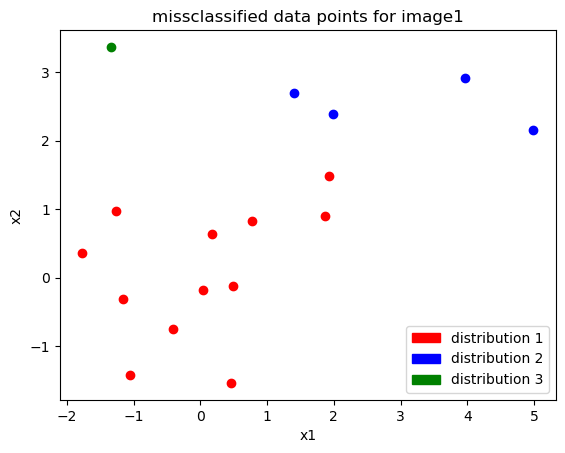
\includegraphics[width=0.33\textwidth]{outputs/output18.png}
    \captionof{figure}{misclassified data points for image1}\label{fig:fig18}
    \splitqsolve
    \centering
    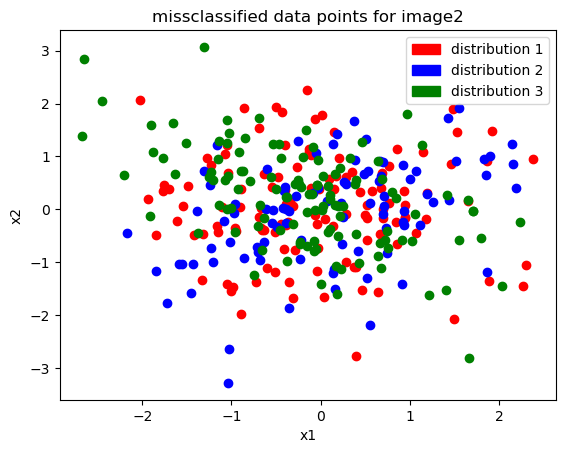
\includegraphics[width=0.38\textwidth]{outputs/output19.png}
    \captionof{figure}{misclassified data points for image2}\label{fig:fig19}
\end{qsolve}
\subsection{Simulation Question 5.}
Compare the parameters obtained from each of the images and explain the reason for their difference.
\begin{qsolve}
    Data from image1 have big difference between mean and also have little variances. So, we can say that data from image1 are less concentrated.That is why, we can see that data from image1 are more spread out than data from image2 nad are easy to separate via EM algorithm.It's also shows that to run EM algorithm for GMM(Gaussian Mixture Model) is more efficient for distributions with small variances and big difference between means.
\end{qsolve}





\makeendpage

\end{document}